\documentclass[11pt,a4paper,oneside]{report}             % Single-side
%\documentclass[11pt,a4paper,twoside,openright]{report}  % Duplex

%\PassOptionsToPackage{chapternumber=Huordinal}{magyar.ldf}
\usepackage{t1enc}
\usepackage[utf8]{inputenc}
\usepackage{amsmath}
\usepackage{amssymb}
\usepackage{enumerate}
\usepackage[thmmarks]{ntheorem}
\usepackage{graphics}
\usepackage{epsfig}
\usepackage{upquote}
\usepackage{listings}
\usepackage{color}
%\usepackage{fancyhdr}
\usepackage{lastpage}
\usepackage{anysize}
\usepackage[magyar]{babel}
\usepackage{sectsty}
\usepackage{setspace}  % Ettol a tablazatok, abrak, labjegyzetek maradnak 1-es sorkozzel!
\usepackage[hang]{caption}
\usepackage{hyperref}
\usepackage{courier}
\usepackage[author={Endre}]{pdfcomment}
\usepackage{float}
\restylefloat{table}


%--------------------------------------------------------------------------------------
% Main variables
%--------------------------------------------------------------------------------------
\newcommand{\vikszerzo}{Galaczi Endre Elek}
\newcommand{\vikkonzulens}{Vajk Tamás}
\newcommand{\vikcim}{Webes gráf- és modellmegjelenítő}
\newcommand{\viktanszek}{Automatizálási és Alkalmazott Informatikai Tanszék}
\newcommand{\vikdoktipus}{Diplomaterv}
%\newcommand{\vikdepartmentr}{}

%--------------------------------------------------------------------------------------
% Page layout setup
%--------------------------------------------------------------------------------------
% we need to redefine the pagestyle plain
% another possibility is to use the body of this command without \fancypagestyle
% and use \pagestyle{fancy} but in that case the special pages
% (like the ToC, the References, and the Chapter pages)remain in plane style

\pagestyle{plain}
%\setlength{\parindent}{0pt} % áttekinthetõbb, angol nyelvû dokumentumokban jellemzõ
%\setlength{\parskip}{8pt plus 3pt minus 3pt} % áttekinthetõbb, angol nyelvû dokumentumokban jellemzõ
\setlength{\parindent}{12pt} % magyar nyelvû dokumentumokban jellemzõ
\setlength{\parskip}{0pt}    % magyar nyelvû dokumentumokban jellemzõ

\marginsize{35mm}{25mm}{15mm}{15mm} % anysize package
\setcounter{secnumdepth}{0}
\sectionfont{\large\upshape\bfseries}
\setcounter{secnumdepth}{2}
\singlespacing
\frenchspacing

%--------------------------------------------------------------------------------------
%	Setup hyperref package
%--------------------------------------------------------------------------------------
\hypersetup{
    bookmarks=true,            % show bookmarks bar?
    unicode=false,             % non-Latin characters in Acrobat’s bookmarks
    pdftitle={\vikcim},        % title
    pdfauthor={\vikszerzo},    % author
    pdfsubject={\vikdoktipus}, % subject of the document
    pdfcreator={\vikszerzo},   % creator of the document
    pdfproducer={Producer},    % producer of the document
    pdfkeywords={keywords},    % list of keywords
    pdfnewwindow=true,         % links in new window
    colorlinks=true,           % false: boxed links; true: colored links
    linkcolor=black,           % color of internal links
    citecolor=black,           % color of links to bibliography
    filecolor=black,           % color of file links
    urlcolor=black             % color of external links
}

%--------------------------------------------------------------------------------------
% Set up listings
%--------------------------------------------------------------------------------------
\lstset{
	basicstyle=\scriptsize\ttfamily, % print whole listing small
	keywordstyle=\color{black}\bfseries\underbar, % underlined bold black keywords
	identifierstyle=, 					% nothing happens
	commentstyle=\color{white}, % white comments
	stringstyle=\scriptsize\sffamily, 			% typewriter type for strings
	showstringspaces=false,     % no special string spaces
	aboveskip=3pt,
	belowskip=3pt,
	columns=fixed,
	backgroundcolor=\color{lightgray},
    literate={á}{{\'a}}1
            {é}{{\'e}}1        
} 		
\def\lstlistingname{lista}	

%--------------------------------------------------------------------------------------
%	Some new commands and declarations
%--------------------------------------------------------------------------------------
\newcommand{\code}[1]{{\upshape\ttfamily\scriptsize\indent #1}}

% define references
\newcommand{\figref}[1]{\ref{fig:#1}.}
\renewcommand{\eqref}[1]{(\ref{eq:#1})}
\newcommand{\listref}[1]{\ref{listing:#1}.}
\newcommand{\sectref}[1]{\ref{sect:#1}}
\newcommand{\tabref}[1]{\ref{tab:#1}.}

\DeclareMathOperator*{\argmax}{arg\,max}
%\DeclareMathOperator*[1]{\floor}{arg\,max}
\DeclareMathOperator{\sign}{sgn}
\DeclareMathOperator{\rot}{rot}
\definecolor{lightgray}{rgb}{0.95,0.95,0.95}
\definecolor{darkgray}{rgb}{.4,.4,.4}
\definecolor{purple}{rgb}{0.65, 0.12, 0.82}
\author{\vikszerzo}
\title{\viktitle}
\includeonly{
	titlepage,%
	declaration,%
	abstract,%
	introduction,%
	chapter1,%
	chapter2,%
	chapter3,%
	chapter4,%
	chapter5,%
	chapter6,%
	acknowledgement,%
	appendices,%
}
%--------------------------------------------------------------------------------------
%	Setup captions
%--------------------------------------------------------------------------------------
\captionsetup[figure]{
%labelsep=none,
%font={footnotesize,it},
%justification=justified,
width=.75\textwidth,
aboveskip=10pt}

\renewcommand{\captionlabelfont}{\small\bf}
\renewcommand{\captionfont}{\footnotesize\it}

%--------------------------------------------------------------------------------------
% Table of contents and the main text
%--------------------------------------------------------------------------------------
\begin{document}
\singlespacing

\pagenumbering{arabic}
\onehalfspacing
%--------------------------------------------------------------------------------------
%	The title page
%--------------------------------------------------------------------------------------
\begin{titlepage}
\begin{center}

\includegraphics[width=60mm,keepaspectratio]{figures/BMElogo.png}\\
\vspace{0.3cm}
\textbf{Budapesti Műszaki és Gazdaságtudományi Egyetem}\\
\textmd{Villamosmérnöki és Informatikai Kar}\\
\textmd{\viktanszek}\\[5cm]

\vspace{0.4cm}
{\huge \bfseries \vikcim}\\[0.8cm]
\vspace{0.5cm}
\textsc{\Large \vikdoktipus}\\[4cm]

\begin{tabular}{cc}
 \makebox[7cm]{\emph{Készítette}} & \makebox[7cm]{\emph{Konzulens}} \\
 \makebox[7cm]{\vikszerzo} & \makebox[7cm]{\vikkonzulens}
\end{tabular}

\vfill
{\large \today}
\end{center}
\end{titlepage}



\tableofcontents\vfill
%--------------------------------------------------------------------------------------
% Nyilatkozat
%--------------------------------------------------------------------------------------
\begin{center}
\large
\textbf{HALLGATÓI NYILATKOZAT}\\
\end{center}

Alulírott \emph{\vikszerzo}, szigorló hallgató kijelentem, hogy ezt a diplomatervet meg nem engedett segítség nélkül, saját magam készítettem, csak a megadott forrásokat (szakirodalom, eszközök stb.) használtam fel. Minden olyan részt, melyet szó szerint, vagy azonos értelemben, de átfogalmazva más forrásból átvettem, egyértelműen, a forrás megadásával megjelöltem.

Hozzájárulok, hogy a jelen munkám alapadatait (szerző(k), cím, angol és magyar nyelvű tartalmi kivonat, készítés éve, konzulens(ek) neve) a BME VIK nyilvánosan hozzáférhető elektronikus formában, a munka teljes szövegét pedig az egyetem belső hálózatán keresztül (vagy autentikált felhasználók számára) közzétegye. Kijelentem, hogy a benyújtott munka és annak elektronikus verziója megegyezik. Dékáni engedéllyel titkosított diplomatervek esetén a dolgozat szövege csak 3 év eltelte után válik hozzáférhetővé.

\begin{flushleft}
\vspace*{1cm}
Budapest, \today
\end{flushleft}

\begin{flushright}
 \vspace*{1cm}
 \makebox[7cm]{\rule{6cm}{.4pt}}\\
 \makebox[7cm]{\emph{\vikszerzo}}\\
 \makebox[7cm]{hallgató}
\end{flushright}
\thispagestyle{empty}

\vfill
\clearpage
\thispagestyle{empty} % an empty page


%----------------------------------------------------------------------------
% Abstract in hungarian
%----------------------------------------------------------------------------
\chapter*{Kivonat}\addcontentsline{toc}{chapter}{Kivonat}

Napjainkban a böngészőben futó webalkalmazások már sok teret hódítottak helyettesítve az asztali alkalmazásokat, hiszen könnyebb a telepítésük, nem kell tárhellyel spórolni és a felhőalapú megoldások bizonyos értelemben biztonságban helyezik az adatainkat. A webes diagramszerkesztő egy jó példa erre, mivel pár percen belül már akár kollaboratívan dolgozhatunk egy diagramon távoli munkatársunkkal.

A szakdolgozatom célja egy webes modellszerkesztő alkalmazás, ami alkalmas vizuális programozásra és kódgenerálásra és ezen felül kollaboratívan lehessen dolgozni benne. Ez a cél mellett a kiválasztott technológiákat is meg kellet ismernem és az elkészült alkalmazást teljesítmény szempontjából értékeltem.

A Javascript reneszánszát éli napjainkban. Már rég nem csak arra való, hogy a böngészőben dinamikus layout-ot létrehozzunk, eljött az a pont, ahol kliens-, szerver- és adatbázis szinten -- idegen szóval -- \emph{full-stack} képességei vannak. A szakdolgozatom keretein belül meg akartam vizsgálni, hogy mennyire érett a technológia komplex webalkalmazások fejlesztésére. 

Munkám eredménye egy kollaboratív diagramszerkesztő, amiben egy kódtranszformációs template-et is megadva tetszőleges nyelvű kódot lehet generálni, Javascript esetében ezt a kódot fel is lehet használni más rendszerben. A kiválasztott technológia alkalmas volt hatékony prototipizálásra, modularitásra és elegáns megoldások implementálására.  

\vfill

%----------------------------------------------------------------------------
% Abstract in english
%----------------------------------------------------------------------------
\chapter*{Abstract}\addcontentsline{toc}{chapter}{Abstract}

Ha jó a magyar, megírom az angolt.
\vfill


%----------------------------------------------------------------------------
\chapter*{Bevezető}\addcontentsline{toc}{chapter}{Bevezető}
%----------------------------------------------------------------------------

Néhány éve foglalkozom Python alapú webfejlesztéssel és munkám során mindig is esztétikusnak tartottam egy könnyen használható de erős keretrendszert. A tapasztalataim elején mindig is óvakodtam a kliensoldali webfejlesztéstől, mert bárhogy csináltam, a jQuery alapú kliensoldali logika a végén sohasem lett olyan szép, mint amire büszke lehetnék. Mire a Javascript tudásom utolérte a Python tudásomat, elburjánoztak a kliensoldali Javascript keretrendszerek amik lehetővé teszik, hogy kliensoldalon is moduláris, tesztelhető és újrafelhasználható megoldásokat alkalmazzak.

A webes modell szerkesztőkre akkor figyeltem fel, amikor a tanulmányaim során a sokadik diagramot kellett megrajzolnom és az akkori Linux rendszeremre nem találtam kielégítő minőségű diagram szerkesztőt. Találtam helyette a Lucidcharts webes eszközt, ami minden akkori próblémát megoldott számomra, ami a diagramszerkesztést illeti.

A vizuális programozásnak az az aspektusa ragadott meg, hogy vannak próblémák amikre egy gráf jellegű megoldás rugalmasabb és átláthatóbb mint a hagyományos kód alapú megoldás és a munkám során próbáltam arra figyelni, hogy olyan vizuális eszközt hozzak létre ami könnyebben old meg próblémákat.

Az MSc szakdolgozatom keretein belül a következőkre terjedt ki a munkám:
\begin{enumerate}
\item Vizuális programozási nyelvek áttekintése és egy vizuális programozási nyelv elkészítése,
\item a kollaboratív diagramszerkesztés megvalósítása, amivel egyidőben több felhasználó tudja ugyanazt a dokumentumot szerkeszteni,
\item a szerveroldali alkalmazás elkészítése, ami perzisztálja az adatokat és támogatja a valósidejű kollaboratív szerkesztést,
\item a HTML5 alapú gráfszerkesztő alkalmazás elkészítése,
\item a megoldáshoz használt technológiák bemutatása, 
\item a megoldás értékelése teljesítmény és skálázhatóság szempontjából.
\end{enumerate}

\clearpage
A fejezetek felépítése a következő:

\begin{enumerate}
\item Az első fejezet a webalkalmazásoknak egy rövid áttekintése, 
\item a második fejezet létező webes diagramszerkesztő, webes programfejlesztő és vizuális programozási nyelveket vizsgál,
\item a harmadik fejezet a kiválasztott technológiákat mutatja be,
\item a negyedik fejezet az elkészült alkalmazás felépítését részletezi mind a szerveroldal és kliensoldali funkciókra kitérve,
\item az ötödik fejezet az alkalmazás teljesítményelemzését mutatja be,
\item az első függelék az alkalmazás telepítését mutatja be Linux rendszeren,
\item a második függelék az alkalmazás felhasználói felületét mutatja be,
\item a harmadik függelék az állapotgép nyelv kódját részletezi.
\end{enumerate}
%----------------------------------------------------------------------------
\chapter{Webes vizuális dokumentumszerkesztők}
%----------------------------------------------------------------------------
(2-3 oldal) 

A Web2.0 világában, amikor a weboldalak továbbfejlődtek az egyszerű statikus tartalom szintjéről elszaporodtak a böngészőben futó alkalmazások. Egy webes dokumentumszerkesztő alatt a böngészőben futó irodai jellegű dokumentum szerkesztőt értjük, az alkalmazás szolgáltatása Saas (Software as a Service) módszerrel történik, amelynél a szoftver és az adatok központilag vannak tárolva és interneten keresztül érhetők el. Manapság a nagyobb szoftvercégeknek a központi stratégiájává vált a SaaS. 
\pdfcomment[icon=Note]{http://peterlaird.blogspot.hu/2008/06/how-oracle-ibm-sap-microsoft-and-intuit.html}

\section{Történet}

1995-ben a Netscape cég bevezette a Javascript kliensoldali szkriptnyelvet, így már lehetséges volt a dinamikus tartalom előállítása anélkül, hogy új kérést küldjön a böngésző a szervernek.

1996-ban a Macromedia cég bevezette a Flash lejátszót, egy vektorgrafikus lejátszót, ami böngésző plug-in-ként volt elérhető.

1999-ben XMLHttpRequest API elérhető volt Internet Explorer 5-ben, lehetséges volt kliens oldalról Javascript kódból egy kérést indítani, ami XML-t kért le a szervertől, majd feldolgozta azt.

2005-ben az AJAX -- Asynchronous Javascript and XML -- fogalom megjelent \pdfcomment[icon=Note]{https://web.archive.org/web/20080702075113/http://www.adaptivepath.com/ideas/essays/archives/000385.php} és ebben az időben Google-nek a Gmail alkalmazásának  funkcionalitása már egyre nagyobb része AJAX alapú volt.

2011-ben érett meg a HTML5, ami multimédia lehetőségeket biztosít a böngészőben plugin-ok nélkül, példáúl video tartalom lejátszására már natív módon van lehetőség. HTML5 Canvas segítségével gazdag két dimenziós grafikus felületek alakíthatók ki. 

\section{Előnyök}

Egy triviális előny az, hogy nem kell az alkalmazást telepíteni a felhasználó számítógépére, természetesen, feltételezve, hogy egy böngésző már telepítve van a rendszeren. Manapság az egyszerű felhasználónak nagy valószínűséggel van telepített böngészője, nem is egy. Ez az előny vállalati szempontból nézve mégnagyobb: egy új vállalati webalkalmazás bevezetése esetében nem kell mind az -- esetleg -- ezer gépre telepíteni szoftvert.
Mégjobb a helyzet amiatt, hogy verzió frissítésnél nem is kell semmit csinálni, a felhasználók megkapják mindig a legújabb verziót. Manapság elterjedtek a kizárólag SSD-t tartalmazó hordozható eszközök, egy 64 gigabájt kapacitású merevlemezre már nem szeretnénk egy több gigabájtos dokumentumszerkesztő készletet telepíteni.

Az elérhetőség egy nagy előny hiszen a felhasználó bármilyen számítógépről -- internet kapcsolatot feltételezve -- el tudja érni az alkalmazást. Ez a centralizáltság adatbiztonság szempontból is előnyös hiszen centralizáltan történik az összes felhasználó dokumentumainak a biztonsági mentése ugyanakkor az átlagos felhasználó leggyakrabban pendrive vagy optikai lemezre menti az adatait, ez előbbit el lehet veszíteni, az útóbbi meg idővel észrevétlenül használhatatlanná válhat. 

A webes tartalmat könnyebb megosztani és könnyebb a kollaboráció.

\section{Hátrányok}

Adatbiztonsági hátrányai vannak viszont a webes dokumentumszerkesztőknek, egyszerűen fogalmazva, annyira biztonságos az interneten tárolt adat amennyire biztonságban van tartva a jelszavunk. Elképzelhető könnyen olyan szituáció, hogy egy jelszót könnyebb megszerezni, mint az otthoni gépen tárolt adatait szerezzük meg valakinek fizikai vagy szoftveres betörés segítségével. Továbbá a bizalmas adataink egy másik cég kezében vannak és nem egyértelmű, hogy mi történik az adatainkkal ha az a cég megszűnik.

Ha sok webes alkalmazást használunk, akkor sok felhasználói fiókot kell létrehozni, a sok fiók nyilvántartása nehézkes lehet egy felhasználónak. Erre alternatíva, példáúl, a Facebook login vagy hasonló megoldás, de akkor az a baj, hogy mi lesz az adatainkkal, ha megszűnik a Facebook fiókunk. 

Egyre kevésbé próbléma, de sokszor nem biztosított az állandó internetkapcsolat és ha nem elég a sávszélesség, akkor esetleg nagyon szenvedhet a használhatóság.



\section{Kihívások}



%----------------------------------------------------------------------------
\section{Kollaboratív alkalmazások}
%----------------------------------------------------------------------------
Derp.




%----------------------------------------------------------------------------
\chapter{Hasonló eszközök vizsgálata}
%----------------------------------------------------------------------------
(10 oldal )Derp derp, valami szöveg. Árvíztűrő tükörfúrógép.


%----------------------------------------------------------------------------
\section{Lucidchart}
%----------------------------------------------------------------------------

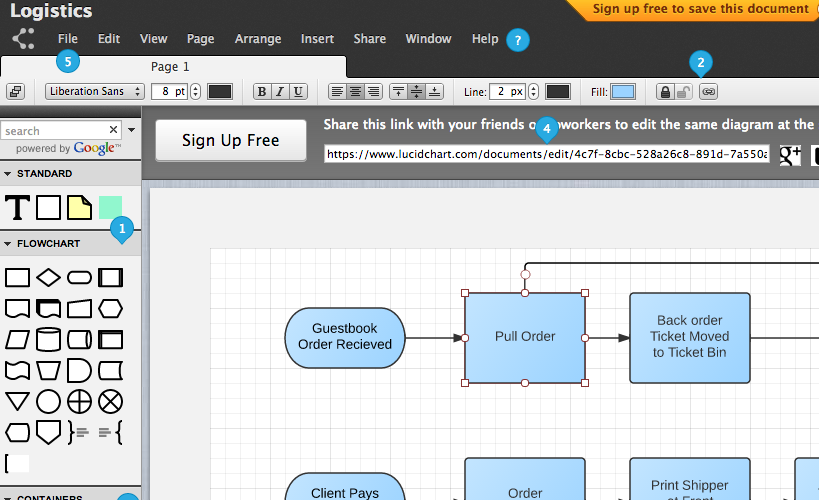
\includegraphics[width=160mm,keepaspectratio]{figures/lucid.png}\\

Lucidchart egy HTML5 és Javascript alapú diagramszerkesztő eszköz. \pdfcomment[icon=Note]{http://lifehacker.com/5112133/lucidchart-makes-stripped+down-flowcharts-for-free} 2008-ban lett béta verzióként elindítva.

 


%----------------------------------------------------------------------------
\section{Gliffy}
%----------------------------------------------------------------------------

Google Chrome plugin-ként offline üzemmódban is működik.


\section{Összefoglalás}





\definecolor{darkgreen}{rgb}{0.2,0.6,0.2}
\lstdefinelanguage{JavaScript}{
  keywords={typeof, new, true, false, catch, function, return, null, catch, switch, var, if, in, while, do, else, case, break},
  keywordstyle=\color{blue}\bfseries,
  ndkeywords={class, export, boolean, throw, implements, import, this},
  ndkeywordstyle=\color{darkgray}\bfseries,
  identifierstyle=\color{black}\bfseries,
  sensitive=false,
  comment=[l]{//},
  morecomment=[s]{/*}{*/},
  commentstyle=\color{purple}\ttfamily,
  stringstyle=\color{darkgreen}\ttfamily,
  morestring=[b]',
  morestring=[b]"
}

\lstset{
   language=JavaScript,
   backgroundcolor=\color{lightgray},
   extendedchars=true,
   basicstyle=\footnotesize\ttfamily\bfseries,
   showstringspaces=false,
   showspaces=false,
   %numbers=left,
   %numberstyle=\footnotesize,
   %numbersep=9pt,
   tabsize=2,
   breaklines=true,
   showtabs=false,
   captionpos=b,
   aboveskip=9pt,
   belowskip=9pt,
}

%----------------------------------------------------------------------------
\chapter{Technológiai áttekintés}
%----------------------------------------------------------------------------
A következő alfejezetekben a felhasznált technológiákra fogok kitérni több hangsúlyt fektetve azokra a technológiákra amik vagy újabbak vagy fontosabb szerepet játszottak az elkészült alkalmazásban.

%----------------------------------------------------------------------------
\section{Javascript}
%----------------------------------------------------------------------------

%A Javascript nyelvet az útóbbi évek fejleményei miatt választottam, hiszen már lehetséges vele egy teljes kliens és szerveroldalt átívelő alkalmazást létrehozni. Szkriptnyelv jellege miatt arra számítottam, hogy gyors prototípizálásra lesz lehetőség, ez azért fontos, mert a technológiák nagy része amivel a diplomunkámban foglalkoztam új volt számomra.

A Javascript nyelv útóbbi évek fejleményei miatt már lehetséges vele egy teljes kliens és szerveroldalt átívelő alkalmazást fejleszteni. Szkriptnyelv jellege miatt gyors prototípizálásra van lehetőség, ez azért fontos, mert sok technológiát kell megismerni a diplomamunka során.

A Javascript nyelv nem kerül részletes bemutatásra, helyette arra tértem ki, ami nehezen érthető volt számomra: az, hogy hogyan tud objektumorientált lenni a nyelv, ha tud egyáltalán. 

\subsection{Prototípus öröklés a Javascriptben}

Javascript egy prototípus alapú objektumorientált nyelv, ez azt jelenti, hogy objektumok vannak, amik nem osztálypéldányok és az öröklés szempontjából minden objektumnak van egy referenciája a prototípusára, és ez addig megy tovább amíg a prototípus null lesz \cite{mdnprotoref}. 

Örökölt attribútumok esetében úgy működik a feloldás, hogy először az objektum saját attribútumai között keressük, ha nem találjuk, akkor a prototípus láncon tovább megyünk és ott keressük, és így tovább a végéig, ahol, ha nem találjuk meg akkor \lstinline{undefined} az eredmény. A függvények attribúmként viselkednek ebből a szempontból és ezáltal a függvény felüldefineálás is működik.

\subsubsection{Objektumpéldányosítás}

Több módon történik az objektumok példányosítása, az egyszerű esetekben a következőképpen néz ki a prototípus lánc: 
\begin{enumerate}
\item \lstinline| var o = { a: 1 };| esetében o az Object-ből örököl és a prototípuslánc:

 \lstinline|o ---> Object.prototype ---> null|
\item \lstinline| var a = ["egy", "meggy", "citrom"]; | esetében az \lstinline{a} egy tömb aminek a prototípusa az Object \lstinline|a ---> Array.prototype ---> Object.prototype ---> null|
\item \lstinline| function foo(){ return 0; }| a függvény is egy ``egyszerű'' objektum: 

\lstinline| foo ---> Function.prototype ---> Object.prototype ---> null| 

\item 
\begin{lstlisting}
{
    function Alma() {
        this.color = "green";
    }
    Alma.prototype = {
        ripe: function() {
            this.color = "red";
        } 
    }
    var a = new Alma();
}
\end{lstlisting}

A konstruktor az egy egyszerű function ami meghívódik a \lstinline{new} kulcsszó használatakor, ekkor a prototípuslánc: 

\lstinline| a ---> Alma.prototype ---> Object.prototype ---> null|

\end{enumerate}

Meg kell jegyezni, hogy a hosszú prototípusláncok teljesítménycsökkentést jelentenek, hiszen végig kell menni mindig a láncon egyes attribútumokért. Az is fontos, hogy a Javascript környezet annyira megengedő, hogy beépített objektumokat lehet változtatni, úgynevezett ``monkey patching''-gel, ez viszont nem javasolt, mert nehéz debuggolni, megnehezíti annak a fejlesztőnek a munkáját aki nem tud a patch-ről és ha két modul ugyanazt a kódot patch-eli, akkor amelyik később inicializálódik az ``nyer''.



\subsection{Coffeescript}

Napjainkban nagyon sok olyan nyelv van ami Javascriptre fordul \cite{coffeeref}. A diplomamunkám elején CoffeeScript-ben fejlesztettem a prototípust, mert egy olyan nyelv ami Javascriptre fordul, de Python jellegű szintaxisa van. A főbb jellegzetességei a következők \cite{maccaw2011}:

\begin{itemize}
\item zárójelek helyett indentálással történik a kód blokkok elválasztása, emiatt olvashatóbb lehet a kód,
\item eltávolítja a globális referencia fogalmát és csak lokális változókat lehet deklarálni,
\item nagyon rövid a függvénydeklaráció: \lstinline|function() { do() ;}| helyett \lstinline{() -> do},
\item nagyon rugalmas ciklusok és lista generálások: \lstinline{[ apple for apple in apples when not apple.rotten ]} ez egy friss alma listával tér vissza egy sorban, 
\item a feltételes blokkok és ciklusok zárójelmentesek és egyszerűbb helyes kódot írni: \begin{lstlisting}
    for i in items
        if i>5 then print i
        \end{lstlisting}
\item nagyon hasznos a feltételes tagváltozóhozzáférés: a \lstinline{apple.tree?.cutDown} kód akkor is sikeresen lefut, ha az \lstinline{apple} objektumnak nincs \lstinline{tree} tagváltozója,
\item bevezeti a Pythonhoz hasonló osztálydeklaráció szintaxist, ami félrevezető lehet, ha nem ismerjük jól a Javascriptet, hiszen csak ezen az absztrakt szinten hagyományos módon értve objektumorientált, a lefordult Javascriptben prototípus öröklés lesz,
\item teljesen ekvivalens Javascript kód fordul belőle és visszafordítás is ugyanúgy lehetséges.
\end{itemize}

Igaz, hogy könnyebb üzleti logikát és funkcionális programozási kihívásokat megoldani a Coffeescript szintaxissal, de azt tapasztaltam, hogy a munkám során nem segített a keretrendszerek (AngularJS, NodeJS) megértésében, nehezebb volt a hibákat debuggolni. Amikor már ismerős volt a technológia, akkor hatékonyabb tudtam lenni Coffeescipt segítségével, de ez csak a végére alakult ki. Egy másik ok az, hogy a jelen dokumentumban sok kódrészlet szerepel és ennek megértését hátráltatja a Coffeescript szintaxis azon olvasó számára aki nem ismeri a nyelvet. 

Bármikor át lehet térni Coffeescriptre hiszen mindkét irányba lehet fordítani, tehát egy létező Javascript projektet Coffeescriptre lehet fordítani, be kell állítani az automatikus fordítást Javascriptre és már dolgozhatunk is tovább Coffeescriptben.


%----------------------------------------------------------------------------
\section{Socket.IO}
%----------------------------------------------------------------------------
A Socket.IO egy JavaScript könyvtár ami valósidejű alkalmazások kétirányú kommunikációját támogatja. Ha a hagyományos kliens-szerver weboldal modellre gondolunk, akkor azt a hiányosságot oldja meg, hogy miután letöltődik a honlap a böngészőben, nem egyértelmű, hogy hogyan tudnánk a kliens oldalon reagálni szerver oldali eseményekre. A WebSocket protokoll egy TCP kapcsolaton full-duplex kommunikációt biztosít.

Valósidejű alkalmazásra egy naív próbálkozás az egyszerű AJAX polling, ami így nézhet ki:
\medskip
\begin{lstlisting}[caption=Egyszerű polling]
setInterval(function(){
    $.ajax({ url: "server", success: function(data){
        //
    }, dataType: "json"});
}, 30000);
\end{lstlisting}

Ez több próblémát is felvet, többek között azt, hogy, ha a polling intervallum túl kicsi, akkor túl sok lekérés megy a szerverhez, ha az intervallum túl nagy, akkor nem kapunk elég gyakran értesítést. Minden egyes lekérdezés egy-egy kapcsolatfelépítést jelentene, ami pazarló lehet.

Erre egy alternatíva a Long Polling, ekkor a válasz nem érkezik meg a szervertől addig, amíg nincsen olyan esemény amiről a klienst értesítenénk:

\begin{lstlisting}[caption=Long Polling]
(function poll(){
    $.ajax({ url: "server", success: function(data){
        // 
    }, dataType: "json", complete: poll, timeout: 30000 });
})();
\end{lstlisting}

Itt is láthatunk néhány hiányosságot: újra kell kapcsolódni periodikusan, mert a kérés lejárhat (timeout) és a kommunikációs protokoll még mindig HTTP, ami overhead-et jelent.


A pollingnál egyszerűbb megoldás egy egyetlen TCP kapcsolatot kialakítani a kétirányú kommunikációra, ezt kínálja a Websocket protokoll \cite{rfc6455}.

A Websocket protokoll arra lett tervezve, hogy a létező kompromisszumos kétirányú megoldásokat helyettesítse. A protokollnak két része van: a handshake és az adatátvitel. Miután végbement a handshake, a két fél \emph{üzenetekben} kommunikál egymással amik \emph{keretekre} lehetnek tagolva.

Ez a keretezés a protokoll saját keretezése és az alsó rétegek akár tovább bonthatják.

A Websocket protokoll egy címzési mechanizmust is megvalósít, amivel több szolgáltatást lehet igénybevenni egy kapcsolaton keresztül.

A kommunikáció a TCP 80 porton történik, ami kedvező akkor amikor tűzfal szűri a többi portot. 




A Socket.IO átlátszó módon kiválasztja a legjobb protokollt az aktuális böngésző által támogatottak közül ebben a sorrendben:
\begin{enumerate}
\item{WebSocket}
\item{Adobe Flash Socket}
\item{AJAX long polling}
\item{AJAX multipart streaming}
\item{Forever Iframe}
\item{JSONP Polling}
\end{enumerate}



Megoldások mint a \url{http://pusher.com} megkönnyítik a Websockets implementációt egy 3rd party szolgáltatás keretein belül, de nem ezt használtam többek között azért mert fizetős szolgáltatás és nem akartam egy külső rendszertől függő alkalmazást fejleszteni.




%----------------------------------------------------------------------------
\section{AngularJS}
%----------------------------------------------------------------------------




Az AngularJS egy nyílt forrású JavaScript keretrendszer ami ``single-page''\footnote{Egy olyan webalkalmazás ami egy weboldalon kifér dinamikusan betöltött tartalommal a jobb felhasználói élmény céljából.} webalkalmazások fejlesztését támogatja. A Google karbantartása alatt van és az első verziója 2009-ben jelent meg. 

\subsection{Kliensoldali HTML generálás}

%\begin{figure}[!ht]
%\centering
%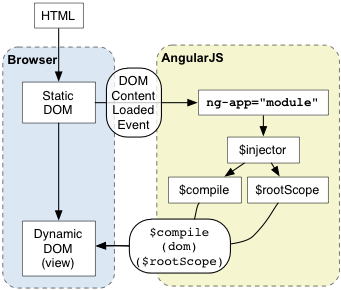
\includegraphics[width=10cm,keepaspectratio]{figures/concepts-startup.png}
%%\caption{Dinamikus kliensoldali HTML AngularJS-ben}
%\label{fig:angularhtml}
%\end{figure}

A hagyományos weboldal esetében a böngészőben megjelenített HTML a szerver oldali alkalmazás által van létrehozva.  A single-page alkalmazás ebben az esetben úgy jön létre, hogy AJAX felhasználásával betöltés után töltődnek be újabb részei az oldalnak\cite{angularbook}. AngularJS esetében ez a művelet a kliens oldalra kerül így a szerver inkább egy adatforrás és statikus tartalom szolgáltatóvá válik. Így lazább csatolást érünk el a szerver és kliens oldal között esetleg párhuzamosítva a fejlesztést és növelve az újrafelhasználhatóságot\cite{AngularDocConcepts}.





\subsection{Direktívák}

Az AngularJS fordító segítségével ki lehet terjeszteni a HTML szintaxist új attribútum és elem típusokkal, ezeket hívják direktívának. 

\lstset{language=HTML}
\begin{lstlisting}[frame=single]  
<ul>
  <li ng-repeat="action in user.actions">
    {{action.description}}
  </li>
</ul>
\end{lstlisting}

Magas szintről nézve a direktívák megjelölik a DOM elemeket és ennek hatására az AngularJS fordító speciális viselkedéssel bővíti ki ezeket az elemeket. A DOM-ot csak direktívák segítségével lehet befolyásolni AngularJS-ben és ez a szeparáció segít a tesztelésben. 

Beépített direktívák vannak, példáúl \lstinline{ng-repeat}, \lstinline{ng-click}, \lstinline{ng-show}, és ezek kiterjeszthetőek saját direktívákkal. Ekkor meg lehet határozni egy HTML templatet a direktívának, ami helyettesíti a DOM-ban a létező elemet az új template-tel és a direktíva \lstinline{link} attribútuma egy olyan függvény ami beállítja fordításkor a kiterjesztett viselkedést példáúl egy jQuery dátumkiválasztót kapcsol a DOM elemhez és ennek eseményeit hozzáköti a modellhez.


\subsection{Model-View-Controller}

Az MVC architektúra a desktop alkalmazások világában lett népszerű és csak az utóbbi években terjedt a webes alkalmazások világába. Az alap ötlet a tiszta elválasztása az adat kezelésnek (modell), az üzleti logikának (kontroller) és a megjelenítésnek (nézet). AngularJS alkalmazásokban a nézet a Document Object Model, a kontrollerek Javascript objektumok vagy függvények, és további objektum attribútumokban van tárolva a model.   

\subsubsection{Adatkötés}

jQuery és hasonló megoldások segítségével újratöltés nélkül frissíteni tudjuk a DOM-ot felhasználói események hatására vagy adatok frissítése esetében, de még az egyszerű esetekben sem biztos hogy triviális a DOM és adatok összehangolása. Az AngularJS ezt két irányú adatkötéssel próbálja megoldani ráadásul deklaratívan. Egy egyszerű példa adatkötésre:

\lstset{language=HTML}
\begin{lstlisting}[frame=single]  
<div ng-controller="HelloController">
  <input ng-model="greeting.text"/>
  <p>{{greeting.text}}, World!</p>
</div>
\end{lstlisting}
Ekkor az input mező módosítása automatikusan a model-t is frissíti és ez a cimkét is frissíti alatta. Ehhez az alap funkcionalitáshoz nem is szükséges más kódot írni.


\subsubsection{Függőséginjektálás}

Függőséginjektálás egy szoftver tervezési minta amiben beégetett függőségek helyett kicserélhető komponenseket használunk amiket akár futás időben is cserélhetünk. 

Ez egység tesztelés esetében válik hasznossá, hiszen jobban lehet izolálni alkalmazás logikát azzal, hogy függőségeket kicserélünk a tesztekben egy úgynevezett ``mocked'' függőséggel. Egy jó példa olyan függőségre amit teszt esetekben ki szeretnénk cserélni egy olyan kódrészlet ami egy különálló rendszernek az API-ját használja ráadásul állapotmódosítással járuló módon, amikor ezt ``mock-oljuk'', akkor tesztelni tudjuk az API felhasználását az API meghívása nélkül.

Egy kontroller a DOM -- vagy a nézet -- egy bizonyos részéhez van kötve, és függőséginjektálás során egy úgynevezett scope kontextus objektumhoz fér hozzá amin keresztül a modellhez férünk hozzá. Ez az elválasztás segít az újrafelhasználásban és karbantarthatóságban, mert, minden kontroller csak azt lát amit kell, hogy lásson és nem ``szennyezzük'' a globális környezetet. 

A scope objektumok egy hierarchiába vannak rendezve, létezik egy gyökér scope, és egymásbaágyazott kontrollerek scope objektumai prototípus örökléssel származnak egymásból.  
 
\begin{lstlisting}
function HelloController($scope) {
    $scope.greeting = {text: "Hello"}
}
\end{lstlisting}

\subsection{Szolgáltatások}

Az AngularJS szolgáltatások egyke példányok, amik bizonyos funkciót valósítanak meg az alkalmazásban, példáúl a \lstinline{http} szolgáltatás egy csomagoló a böngésző XMLHttpRequest objektuma körül és vele lehet AJAX hívásokat végrehajtani. 

AngularJS szolgáltatásokat injektálni kell, mint minden más függőséget, egy komponensbe, példáúl tudunk injektálni kontrollerbe, direktívába, szolgáltatásba stb. Természetesen saját szolgáltatást is lehet fejleszteni és ajánlott is az újrafelhasználandó logikát egy ilyen szolgáltatásba helyezni.

A kontrollerekbe mindig injektálni kell a \lstinline{scope} szolgáltatást, így megvalósul a kapcsolat a modell és a kontroller között.


%----------------------------------------------------------------------------
\section{MongoDB}
%----------------------------------------------------------------------------

A MongoDB egy nyílt forráskódú dokumentum-orientált adatbázis rendszer. A MongoDB nem egy relációs adatbázis, nem lehet SQL nyelv segítségével lekérdezéseket futtatni, nem támogat JOIN műveletet. A MongoDB BSON\footnote{Binary JSON} formátumban tárol kulcs-érték párokat. Az RDBMS\footnote{Relational Database Management System} alapfogalmai: adatbázis, tábla, sor, oszlop; a MongoDB megfelelői: adatbázis, kollekció, dokumentum, mező. Egy mező értéke lehet egszerű típus, lista vagy beágyazott dokumentum. A dokumentumok nem támogatnak sémát, tehát azonos fajta információnak lehet eltérő sémájú tartalma. 


\subsection{Indexelés}

MongoDB egy relációs adatbázishoz hasonlóan támogat indexelést, erre egy példa az~\ref{sec:dbprof} fejezetben lesz bemutatva. Érdekes fogalom a ``compound'' vagyis összetett index, ennek segítségével több mezőre is lehet egyszerre indexet építtetni és egy olyan lekérdezés ami egy termék gyártója és típusa alapján szűkít hatékony tud lenni.

Egy másik érdekes index fajta a ``multikey'' index, ami lehetővé teszi, hogy egy tömb értékű mező elemeit is indexeljük. Ha egy blogbejegyzés rekordban a bejegyzést kedvelő felhasználók tömbje van, akkor indexek támogatásával tudunk hatékony lekérdezéseket futtatni, példáúl szűrni az olyan bejegyzéseket, amiket Laci kedvelt.

\subsection{Replikáció}

A MongoDB egyik előnye, hogy nagyon könnyű benne adatbázisreplikációt megvalósítani. Egy replika halmaz több adatbázist tartalmaz aminek az egyik tagja a fő adatbázis ami elfogad írás műveleteket és a többi tag megkap minden változást és csak olvasás műveletet lehet rajtuk végrehajtani. A fő csomópont kiesése esetében a többi csomópont megszavaz egymás közül egy csomópontot aki átvegye a fő csomópont szerepét. Amikor a régi csomópont feléled, akkor szinkronizálja a változásokat és újra átveszi régi szerepét.

Az a kényelmes, hogy a kapcsolódó adatbázismeghajtók automatikusan kiválasztják a legközelebbi csomópontot az olvasáshoz. A közelség itt nem földrajzilag értendő, hanem a hálózati késleltetésre vonatkozik, sokszor összefügg a kettő. A csomópont szavazások és új szerepek kiosztásával nem kell foglalkoznia a fejlesztő aki kapcsolódik egy replika halmazhoz. 

\subsection{Sharding}

Egy nagyon sok adattal dolgozó rendszer túlterhelhet egy MongoDB adatbázist és ezt lehet egy darabig függőleges skálázással orvosolni, vagyis több fizikai erőforrást biztosítunk az adatbázisnak, de a terhelés állandó növekedése mellett csak időt nyerünk vele. 

Ehelyett a MongoDB vízszintes skálázhatóságot tesz lehetővé ``sharding'' segítségével. Ekkor az adatok partícionálása történik meg, a különböző partíciók különböző adatbázisokból lesznek elérhetőek. Az adatok partícionálása egy rögzített mező mentén történik, ezt később nem lehet megváltoztatni. Példáúl egy dokumentumszerkesztő rendszerben érdemes partícionálni a dokumentum tulajdonosa mentén, ekkor egy adatbázisra nézve csökken az írási és olvasási műveletek átlagszáma, ha egy felhasználó munkafolyamatot indít akkor csak az egyik adatbázis partícióban fog dolgozni.

A partícionáló rendszer próbál egyensúlyozottan partícionálni és, ha az egyik partíció megnő a többihez képest, akkor átlátszó módon átmozgat rekordokat egy másik partícióba.

A sharding és a replikáció egyszerre használható és kombinálható, példáúl három partíciónk lehet és mind a háromban három-három replika halmazunk lehet, így összesen kilenc csomópontunk lesz.



\subsection{ACID}

Fontos megjegyezni, hogy a RDBMS rendszerekkel szemben a MongoDB nem tud ACID trazakciókat biztosítani \cite{acidref}. 
\begin{enumerate}
\item{Atomicitás}: csak dokumentum szintű atomikus műveletek biztosítottak, ha több kollekció vagy dokumentumon átívelő atomikus tranzakciókat szeretnénk, akkor vagy használjunk RDBMS-t, vagy saját magunk kell egy zárolási mechanizmust fejleszteni.
\item{Konzisztencia}: replikáció esetében a fő adatbázis csomópontot érintik az írás műveletek, az olvasás műveletek meg -- opcionálisan --  a ``közelebb'' tartózkodó csomóponthoz fordulnak. Ebben az esetben ``eventual consistency''-ről beszélünk és nem biztosított, hogy friss adatot olvasunk.  
\item{Izoláció}: MongoDB esetében nem lehet beszélni izolációról, mert csak dokumentumszintű tranzakciók vannak és minden dokumentum művelet hatása azonnal elérhető a többi folyamat számára. 
\item{Tartósság}: teljesítmény árán lehet a tartósságot növelni, példáúl úgy, hogy egy írás művelet a többi csomópontra is íródjon mielőtt visszatérne.
\end{enumerate}

%A CAP\footnote{(C)onsistency - Konzisztencia, (A)vailability - Elérhetőség, (P)artition tolerance - Partícionálás tolerancia} tétel kijelenti, hogy egy elosztott rendszer nem tudja egyszerre teljesíteni a ...

A 32 bites rendszereken a mongoDB szerver csak 2GB tárral gazdálkodhat, ugyanakkor a 64 bites esetben csak a hardver mérete korlátozza.










%----------------------------------------------------------------------------
\section{Node.JS}
%----------------------------------------------------------------------------

Node.js egy Javascript alapú platform amivel skálázható szerveroldali alkalmazásokat hoznak létre és a Google V8 Javascript motorra épül. Node.js egy webszerver modult is tartalmaz aminek segítségével önmaga is tud webszerverként működni. A platform alapítója azzal a céllal hozta létre a Node.js-t hogy egyszerűen lehessen olyan weboldalakat létrehozni amik képesek kétirányú kommunikációra és én is ezért választottam mint szerver oldali technológia ugyanis a legkönnyebben integrálódik a Socket.IO rendszerrel.  Egy másik ok az, hogy nagyon könnyen lehet benne prototipizálni.



\subsection{Nem-blokkoló IO}

A legfeltűnőbb sajátossága a Node.JS platformnak az, hogy majdnem semmilyen hívás nem blokkoló és elsőre elég furcsa csupa aszinkron függvényekkel dolgozni. Ebben rejlik a Node.JS skálázhatósága, ahelyett hogy szálakat allokáljon HTTP kérésekhez, amik drágák és nem lehet belőlük nagyon sok, aszinkron módon az operációs rendszertől vár értesítést, hogy van egy bejövő kérés és addig alszik. A Nem-blokkoló IO abban segít, hogy sohasem vár egy erőforrásra, hanem , példáúl, adatbázis lekérdezést indít, kiszolgál néhány más kérést és később megérkezik az adatbázistól a kért adat. 

Ennek egy következménye az úgynevezett ``shared-state concurrency'' amiben a különböző kérések kiszolgálása nem külön folyamat vagy szálban fut, így egy memóriabeli változó megváltozhat a hívás és a callback lefutása között egy másik kérés által. Erre tipikus ellenpélda az Apache szerver ami minden kérésre új szálat indít friss állapottal. Mivel egy folyamatban fut a Node szerver, lehetséges blokkolni a szervert példáúl azzal, hogy egy callback-ben nagy számot faktorizálunk. Node valójában nem valósít meg konkurrenciát hiszen egyszerre csak egy függvény fut, de mivel ezek gyorsan futnak V8 alatt és nem blokkolnak ezért hatékonyan tud átlagos hardveren több ezer lekérdezést kiszolgálni másodpercenként\cite{nodebook}.

\subsection{Modulkezelés}

A böngésző világában egy külső Javascript könyvtár használatánál -- példáúl a gyakori \lstinline|<script src='http://code. jquery.com/jquery-1.6.0.js'>| -- valószínű, hogy a globális névtérbe kerülnek az új deklarált változók. A jQuery a ``\$'' változót deklarálja a globális névtérben, és ha beteszünk egy másik modult ami ugyanezt csinálja, akkor az első nem fog már működni. 


A szerveroldali Javascript világában az npm\footnote{Node Packaged Modules} segítségével kell 3rd party modulokat telepíteni és egyidejűleg izolált környezetet biztosítani a különböző projekteknek. A Python világában a virtualenv az eszköz amivel lehet izolált környezetet biztosítani és mellette a pip parancs segítségével lehet modulokat telepíteni. Virtualenv-vel szemben az npm alapértelmezetten a lokális környezetünkbe telepít modulokat, virtualenv esetében ez fordítva van, ez néha zavaró, ha a fejlesztő elfelejti aktiválni a környezetet és rossz környezetbe települ a csomag.
Az npm továbbá abban is segít, hogy egy telepített függőséget lehetséges egyből bele is íratni a függőségleíróba:
\lstset{language=bash}   
\lstinline{npm install --save express}.
Ez a függőség leíró a package.json fájl és \lstinline{npm install} paranccsal (paraméter nélkül) minden függőség települ. Ez nem csak a rendezettség miatt fontos, hanem amiatt is, hogy sok node webhosting megoldás -- többek között az általam használt nodejitsu\footnote{http://www.nodejitsu.com} -- a package.json csomagjait telepíti az alkalmazásunkhoz.   

A csomagok a require modul segítségével töltődnek be dinamikusan, példáúl
\begin{lstlisting}
var fs = require('fs');
\end{lstlisting}





%----------------------------------------------------------------------------
\section{MEAN stack}
%----------------------------------------------------------------------------

%http://blog.mongodb.org/post/49262866911/the-mean-stack-mongodb-expressjs-angularjs-and

A MEAN, a MongoDB, ExpressJS, AngularJS, NodeJS technológiáknak a rövidítése, és a lényege az, hogy adatbázisban, szerver oldalon és kliens oldalon végig JSON objektumokkal dolgozunk ráadásul nincs is szükség még más keretrendszerre weblapok készítéséhez, ez egy úgynevezett ``full-stack'' megoldás. A MEAN előnye az, hogy a kölönböző rétegekre specializált fejlesztők akik egy ilyen fejlesztésen dolgoznak könnyebben megértik a többi réteg kódját, hiszen Javascript nyelven történik mindháromnak a fejlesztése. 


\section{Felhasznált fejlesztői eszközök}

Ebben a fejezetben azokat a fejleszői és dokumentáló eszközöket mutatom be röviden amiket diplomamunkámhoz felhasználtam.

\subsection{Jetbrains Webstorm}

A Javascript kódot Jetbrains Webstorm fejlesztőkörnyezetben szerkesztettem. A fő okok amiért ezt választottam:
\begin{itemize}
\item bizonyos mértékben támogat ``IntelliSense'' jellegű kódkiegészítést és kódvalidálást, ami szkriptnyelvek esetében elég hasznos,
\item lehet vele debuggolni egy NodeJS szerveralkalmazást,
\item támogat kódnavigálást.

\end{itemize}

\begin{figure}[!ht]
\centering
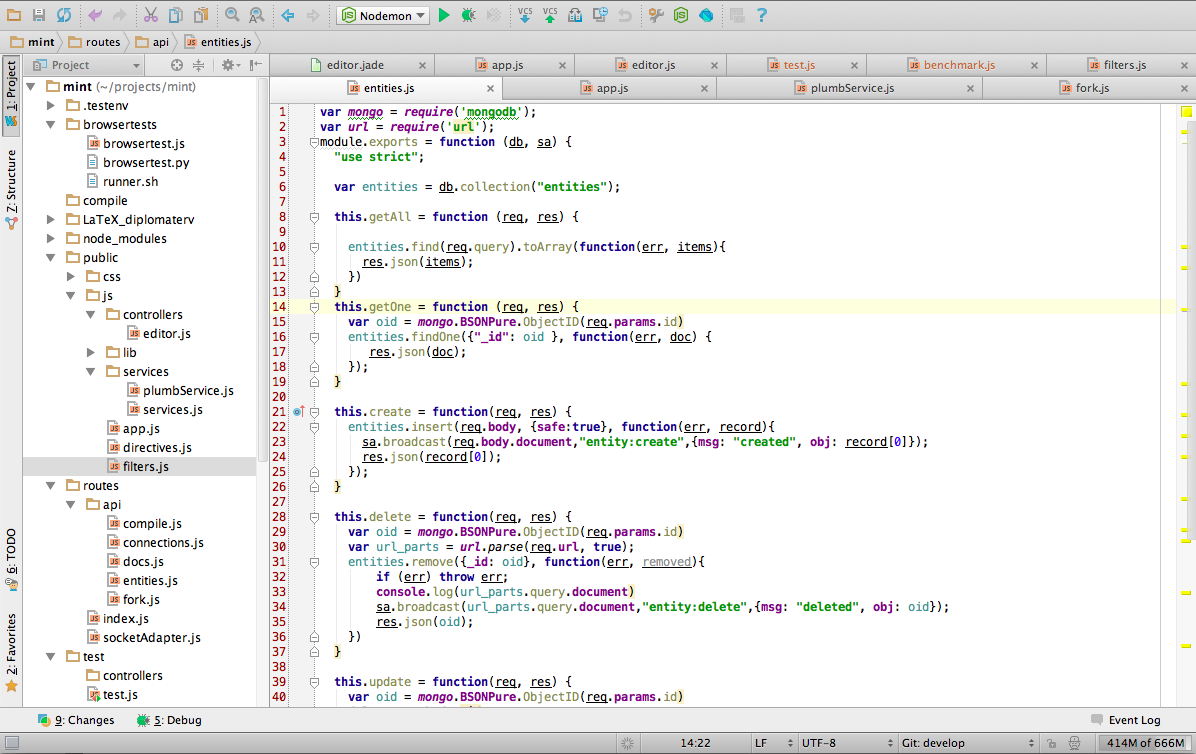
\includegraphics[width=15cm,keepaspectratio]{figures/webstorm.png}
\caption{Jetbrains Webstorm}
\label{fig:webstorm}
\end{figure}

\subsection{Chrome Developer Toolbar}

Az alkalmazásomat fejlesztés közben Google Chrome-ban próbáltam ki főleg a fejlesztői panel miatt, amivel beállítva egy breakpointot vagy a \lstinline{debugger} sor beszúrásával hatékonyan lehet debuggolni. Ráadásul a breakpointnál megállva a Javascript shell az aktuális kontextusban működik és lehet azt a kontextust manipulálni parancsok beírásával.


\subsection{Node Inspector}

A Node Inspector eszköz\footnote{ \url{https://github.com/node-inspector/node-inspector} címről szerezhető be} egy olyan szerveralkalmazás amivel egy Chrome Developer Toolbar példányt a NodeJS szerveroldali alkalmazáshoz lehet csatolni és ugyanazt a debuggolási funkcionalitást lehet elérni szerveroldalon mint kliensoldalon. Sokszor kényelmesebb volt ezt használni a Webstorm debuggernél.

\subsection{Wireshark}

A Wireshark protokollanalizátort a Websocket forgalom vizsgálására volt hasznos amit a~\ref{sec:simprof} fejezetben részletezek.

\subsection{Lucidcharts}

A rendszerábrákhoz Lucidcharts szerkesztőt használtam, mert hatékonyan lehet benne jó minőségű ábrákat gyártani.

\subsection{Latex}

A jelen szöveges dokumentumot Latex-ben írtam a diplomaterv portál sablonját felhasználva. Elég sok időbe került amire mindent beállítottam, de a következő okok miatt találtam nagyon hatékony eszköznek:

\begin{itemize}
\item A dokumentumot fel lehet darabolni több fájlba, akár több mélységben is, majd a fordító összefésüli,
\item nem valószínű, hogy lokális módosítások elrontják a dokumentum egy másik részét,
\item az ábrák egy helyre vannak gyűjtve, ki tudok cserélni egy ábrát úgy, hogy ne kelljen megnyitanom a szerkesztőt,
\item kevésbé valószínű, hogy a Notepad jellegű szövegszerkesztőm lefagy Latex forrás szerkesztése közben, mint az, hogy egy bonyolultabb szövegszerkesztő lefagyjon,
\item könnyebbnek találtam az ábrák beszúrását és testreszabását.
\end{itemize}

Sokszor nehéz debuggolni, hogy miért nem fordul le a dokumentum.

\subsection{Git}

Fontos volt, hogy a munkám ne vesszen el, így egy Git repository-ba tettem, amit egy szerverre szinkronizáltam rendszeresen. A szöveges dokumentumot is beletettem a repository-ba, így a teljes munkám előző állapotait is tudtam böngészni.




%----------------------------------------------------------------------------
\chapter{Az elvégzett munka}
%----------------------------------------------------------------------------
Derp derp, valami szöveg\cite{Wettl04}. Árvíztűrő tükörfúrógép.


%----------------------------------------------------------------------------
\section{Árvíztűrő tükörfúrógép}
%----------------------------------------------------------------------------
Derp.




%----------------------------------------------------------------------------
\chapter{Teljesítményelemzés és optimalizálás}
%----------------------------------------------------------------------------

(3-4 oldal)

Derp derp, valami szöveg. Árvíztűrő tükörfúrógép.

Selenium tesztek


%----------------------------------------------------------------------------
\section{Kollaborációs teljesítményelemzés}
%----------------------------------------------------------------------------


%----------------------------------------------------------------------------
\subsection{Szimuláció}
%----------------------------------------------------------------------------
\label{sec:simprof}

A szimuláció célja automatizálni a felhasználói bemenetet egy teljesítmény méréshez. A megoldásnak tartalmaznia kell alapszintű felhasználói bemenet szimulálását: egérkattintás, szövegbeírás, várakozás és mivel egy grafikus modellt akarunk szerkeszteni a ``drag and drop'' funkcióra is szükség van. 

A böngészőautomatizálás Selenium Webdriver segítségével történt, ez az eszköz lehetővé teszi, hogy különböző nyelveken megírt (Python, Java, PHP stb. ) teszt esetekben a Webdriver API-val kommunikálva böngésző példányokat lehet irányítani. 
Seleniumhoz tartozik egy grafikus fejlesztőkörnyezet is ami Selenium IDE néven Firefox böngészőkiegészítésként fut, vele rögzíteni lehet felhasználói bemenetet és egér eseményeket, majd egy ilyen felvételt újralejátszani, módosítani. Ez előnyös teszterek számára akik repetitív munkát végeznek és nem tudnak programozni, de fejlesztők számára is jó, mert ezekből a felvételeket Python, Ruby stb teszteseteket lehet exportálni. 
Azon kívül, hogy automatizált tesztelésre a szkriptek alkalmasabbak, a Selenium IDE sajnos nem tud egérmozgatást rögzíteni, így nem hasznos a feladat szempontjából. A Selenium API javascript implementációját példáúl a selenium-webdriver csomag valósítja meg, viszont hamarosan kiderült, hogy ez a csomag nem támogatja ``drag and drop'' funckciót, emiatt a Python implementációt választottam. 

A fejlesztés korábbi stádiumában meg kellett győződni, hogy az alkalmazás valamennyire tűri a rossz internetkapcsolatot, ezért egy teszt környezetet alakítottam ki amiben két felhasználót szimulálva két selenium szkript ugyanazt a dokumentumot szerkeszti és véletlenszerű változtatásokat hajt végre a diagramon, pontosabban véletlen entitást mozgat el véletlen irányba. Az elvárt eredmény az, hogy rossz internet kapcsolat mellett is sok idő elteltével ugyanazt a diagramot látja a két felhasználó és azt, hogy ``ugyanazt'' a diagramot látják a diagram hash megegyezése igazolja.
 

\begin{figure}[!ht]
\centering
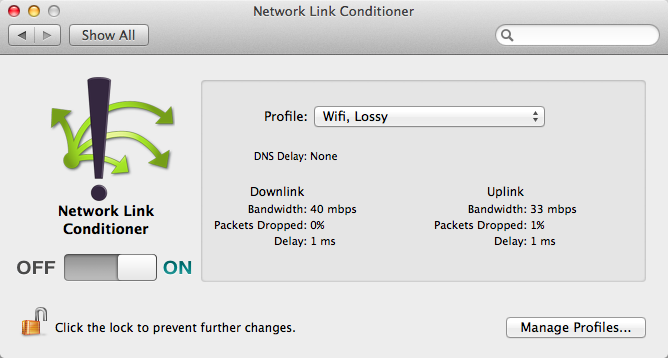
\includegraphics[width=15cm,keepaspectratio]{figures/nlc.png}
\caption{OSX Network Link Conditioner}
\label{fig:nlc}
\end{figure}


A rossz internet kapcsolat szimulálásához OSX-en a Network Link Conditioner alkalmazást használtam, ami az XCode fejlesztőkörnyezet egy kiterjesztése. A felhasználói felülete elég egyszerű és maximálisan megfelel a funkcionalitása a szimulációhoz, ezen kívül a létező profilok is hasznosak, ha példáúl egy gyenge jelű 3G kapcsolatot akarunk szimulálni. A paraméter amire kiváncsi voltam az a csomagvesztési arány volt, úgy azt kezdtem állítani egyre magasabb értékre. Az eszköz bekapcsolása után a ping parancssoros eszköz segítségével egy publikus ip-t pingelve\footnote{példáúl \lstinline{ping www.google.com}} kipróbáltam, hogy valóban akkora a csomagvesztés.

Az eredmény meglepő volt: már olyan csomagvesztési aránynál, ami nekem kicsinek tűnt, példáúl 10-20\% ?????nem lehetett bongeszni????
de a diagram egyezett a két felhasználónak. Wireshark protokolanalizátor segítségével megvizsgáltam, hogy ez miért is lehet, hogy nem veszett el esemény:


\begin{figure}[!ht]
\centering
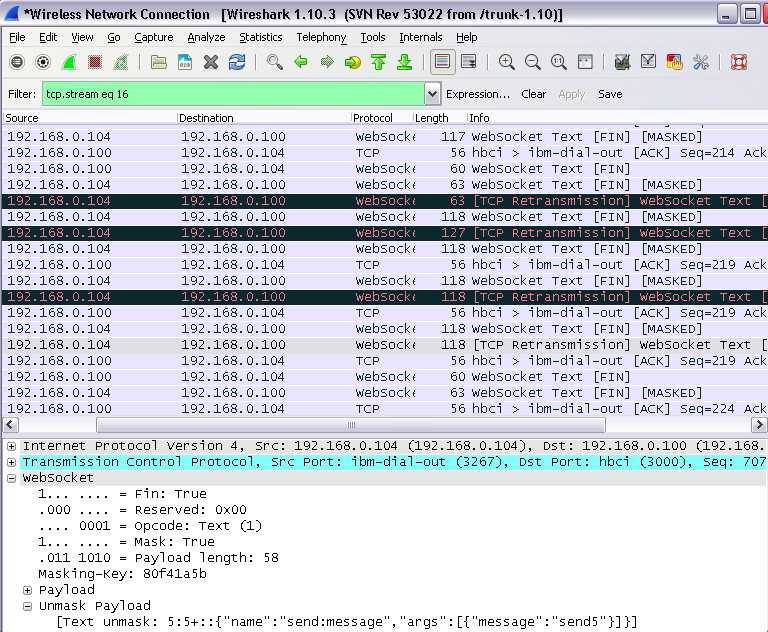
\includegraphics[width=15cm,keepaspectratio]{figures/wireshark.png}
\caption{A Websockets forgalom vizsgálata Wireshark segítségével}
\label{fig:wireshark}
\end{figure}


Wireshark-ban a Websockets protokoll-ra filtereltem, és egy újraküldött csomagra kattintva (a fekete sorok egyike) megnéztem az adott TCP folyamot. Látszik, hogy 192.168.0.104 -- a kliens ebben az esetben -- websockets üzeneteket küld, és a szerver TCP nyugtát küld (ACK) és amikor ez nem történik meg, akkor újraküldődik az üzenet.



++++++++++++++++++++++++
random módon két ember crudol és le kell mérni , hogy mennyire valószínű, hogy elvésznek a bemenetei
++++++++++++++++++++++++

%----------------------------------------------------------------------------
\section{Kliens oldali teljesítményelemzés}
%----------------------------------------------------------------------------
Derp.

A deep watching teljesitmenyelemzése

%----------------------------------------------------------------------------
\section{Webszerver teljesítményelemzés}
%----------------------------------------------------------------------------
Derp.

%----------------------------------------------------------------------------
\section{Adatbázis teljesítményelemzés}
%----------------------------------------------------------------------------
\label{sec:dbprof}
Vizsgáljuk meg, hogy csupán az adatbázis szint hogy viselkedik a terhelés szempontjából. Két kollekció van a dokumentumok és az entitások kollekciója. MongoDB shellből megvizsgálva a kollekcióimat vissza is igazolódik amit sejtettem, hogy a kollekciókon van indexállomány az elsődleges kulcson. A mongoDB shell az majdnem egy NodeJS shell, csak az adatbázis műveletei szinkronok és néhány nem-Javascript parancsot is támogat, példáúl:

\begin{itemize}
\item \lstinline{show dbs} -- az adatbázisok listázása
\item \lstinline{use <db> } -- adatbázis kiválasztása  
\item \lstinline{show collections} -- kollekciók listázása
\item \lstinline{show users} -- adatbázis felhasználók listázása
\end{itemize}

\begin{lstlisting}[caption=A diagram kollekció indexei]
> db.docs.getIndexes()
[
    {
        "v" : 1,
        "key" : {
            "_id" : 1
        },
        "ns" : "mint.docs",
        "name" : "_id_"
    }
]
\end{lstlisting}

Mivel a kliensoldali alkalmazás azonosító -- vagy elsődleges kulcs -- alapján kérdezi le a diagramokat, fölösleges ezzel a kollekcióval kezdeni az elemzést. Érdekesebb az \lstinline{entities} kollekció, ott nem azonosító alapján történik a lekérdezés, amikor egy diagramhoz a tartalmazott entitásokat kérjük.
Nézzünk meg egy ilyen lekérdezést a MongoDB shellben:

\begin{lstlisting}[caption=Az diagram kollekció egy lekérdezésének a query terve]
> db.entities.find({document:"52a37e129deb89c9bd0678aa"}).explain()
{
    "cursor" : "BasicCursor",
    "isMultiKey" : false,
    "n" : 200,
    "nscannedObjects" : 370,
    "nscanned" : 370,
    "nscannedObjectsAllPlans" : 370,
    "nscannedAllPlans" : 370,
    "scanAndOrder" : false,
    "indexOnly" : false,
    "nYields" : 0,
    "nChunkSkips" : 0,
    "millis" : 0,
    "indexBounds" : {

    },
    "server" : "Endres-Laptop-54.local:27017"
}
\end{lstlisting}


A [?] példában nem a lekérdezést lehet látni, hanem a lekérdezés tervet. Ez a terv sok fontos információval szolgál, ha optimalizálni akarunk:

[reference http://docs.mongodb.org/manual/reference/method/cursor.explain/]

\begin{itemize}
                        
  \item{cursor} - A kurzor típusa, amivel lefutott a query. Ha ez \lstinline{BasicCursor} akkor az adatbázis a teljes kollekciót beolvasta a query kiértékeléséhez, tipikusan akkor, ha nem tudott semmilyen indexet felhasználni a lekérdezéshez.
  \item{isMultikey} -  Olyan mezőket is lehet indexelni, aminek az értéke egy tömb. Példáúl \lstinline|{a: 1, b : [1,2,3,4]}| dokumentumok esetében lehetséges a \lstinline{b} tömb elemeit is indexelni. 
  \item{n} - A találatok száma. A fenti példában ez 200.
  \item{nscanned} - A dokumentumok száma ami meg lett vizsgálva, a query kiértékeléséhez. Arra kell törekedni, hogy a \lstinline{n} és a \lstinline{nscanned} közel legyenek egymáshoz. A fenti példában ez 370.

   \item{scanAndOrder} - Ez akkor \lstinline{true}, ha az adatbázis nem tudta felhasználni az indexet rendezésre és a találatokat újra kelett rendezni.
   \item{indexOnly} - Lehetséges olyan indexet felépíteni -- compound index -- ami több attribútumra vonatkozik egyszerre és ha az összes attribútuma a találatoknak benne volt az indexben, akkor az index ``fedi'' a queryt és csak az index alapján értékelődött ki. 
   \item{nYields} - A lekérdezés során hányszor kellett feloldani az olvasás zárat ahhoz, hogy egy másik írás query megtörténhessen. 
   \item{millis} - A lekérdezéshez szükséges ezredmásodpercek száma.


\end{itemize}

Amikor 370 rekord van a kollekcióban akkor elég gyorsan lefut a lekérdezés, gyakorlatilag azonnal, de vizsgáljuk meg hogy alakul ez amikor több rekord van és ugyanazt a 200-at kérdezzük le:


\begin{table}[H]
\centering
\begin{tabular}{|c|c|}

%content goes here
\hline
Rekordok száma & Lekérdezési idő ezredmásodpercben \\
\hline
370 & 0 \\
2000 & 0 \\
20000 & 11 \\
200000 & 89 \\
500000 & 220 \\
1000000 & 447 \\
2000000 & 907  \\
\hline
\end{tabular}
\caption{Lekérdezési idő alakulása az összes rekord száma szerint } 
\end{table}

Látszik, hogy elég sok rekordnál, egy diagram elemeinek lekérdezése már másodperc nagyságrendű időbe telik. Ez még tolerálható lehetne, mert 10000 felhasználóig valószínüleg 2000000 alatt maradna az összes entitás száma és a lekérdezések nagy része úgyis elsődleges kulcs alapú -- ami gyors. A 10000-es nagyságrendet meghaladva felhasználó számban (feltéve, hogy átlagban egy felhasználó 100 elemet hoz létre összesen) már túl lassúnak bizonyulna ez a megoldás.

Megvizsgáltam mennyire hatékony lehet a megoldás erre a próblémára, nyilvánvalóan indexelni kell a \lstinline{document} attribútumás az entitás kollekciónak és ez a következőképpen történik a MongoDB shellben:

\begin{lstlisting}[caption=Index létrehozása]
> db.entities.ensureIndex({document: 1})
> db.entities.getIndexes()
[
    {
        "v" : 1,
        "key" : {
            "_id" : 1
        },
        "ns" : "mint.entities",
        "name" : "_id_"
    },
    {
        "v" : 1,
        "key" : {
            "document" : 1
        },
        "ns" : "mint.entities",
        "name" : "document_1"
    }
]
\end{lstlisting}

A \lstinline{getIndexes()} paranccsal ellenőriztem, hogy tényleg létre is jött az index. Újból \lstinline{.explain()}-vel indítva lekérdezést a query tervben látszik, hogy \lstinline{"cursor" : "BtreeCursor document_1"}, tehát már az új indexet használja fel a kereséshez, ráadásul, a megvizsgált rekordok száma megegyezik a találatok számával. 

Nem meglepő, hogy 2000000 rekord esetén is majdnem egy másodperc helyett -- index segítségével -- 0 ezredmásodpercet jelez a query terv. Azt is meg lehet vizsgálni, hogy ez a kényelem mennyibe kerül és ezt a \lstinline{db.entities.stats()} paranccsal lehet megtudni:

\begin{lstlisting}[caption=Kollekció és index nagysága]
> db.entities.stats()
{
    "ns" : "mint.entities",
    "count" : 2000370,
    "size" : 208047512,
    "avgObjSize" : 104.00451516469454,
    "storageSize" : 243314688,
    "numExtents" : 13,
    "nindexes" : 2,
    "lastExtentSize" : 68579328,
    "paddingFactor" : 1.0000000000000022,
    "systemFlags" : 1,
    "userFlags" : 0,
    "totalIndexSize" : 177672656,
    "indexSizes" : {
        "_id_" : 64917440,
        "document_1" : 112755216
    },
    "ok" : 1
} 
\end{lstlisting}

Ebből kiderül, hogy 200MB az adat mérete és emellett az index mérete 178MB, tehát az összes tárhely majdnem a felét a két index foglalja el. Ennek az a magyarázata -- többek között -- hogy kevés adatot tárolunk egy rekordban, ami az \lstinline{avgObjSize} eredmény szerint 100 bájt. Az entitásokat kibővítve új adatokkal, példáúl színnel, szerencsére nem fog nőni az index mérete és kedvezőbb lesz a tárfoglalási arány.



%----------------------------------------------------------------------------
\chapter{Összefoglalás és továbbfejlesztés}
%----------------------------------------------------------------------------

A diplomamunkámmal elértem a kitűzött célt: létező kollaboratív alkalmazás vizsgálata alapján megterveztem egy olyan rendszert, ami több felhasználónak teszi lehetővé, hogy egyidőben dolgozzanak egy diagramon. Emellett a felhasználó egy vizuális nyelvet is létrehozhat egy transzformáció megírásával, majd a generált kódot fel is használhatja. 

Teljesítmény szempontjából a kollaboráció elég jól működik és a webszerver és adatbázis is megfelelően jól teljesít, a felhasználói élményen lehet még javítani és jelen állapotában -- kliensoldali teljesítménypróblémák miatt -- 100 elemszám alatt jól lehet használni.

További pozitív eredmény az, hogy akár a továbbfejlesztések nélkül is a rendszer alkalmazható más rendszerek modellezési próblémáinak megoldására. 

A munka sikeres abból a szempontból is, hogy a MongoDB, NodeJs és AngularJS technológiákból felépített prototípus, majd teljes alkalmazás izgalmas, kényelmes és tanulságos volt fejleszteni. A jövőben mindenképpen fel fogom használni az említett technológiákat.





%----------------------------------------------------------------------------
\section{Továbbfejlesztési lehetőségek}
%----------------------------------------------------------------------------

A következő alfejezetekben azokat az ötleteket gyűjtöm össze amik számomra a továbbfejlesztési irányokat jelentik, hiszen bízom benne, hogy a jövőbeli munkám során hasznos lehet a szakdolgozat alatt fejlesztett alkalmazás.

\subsection{Vizuális modellezés kibővítése új elemekkel}

Sok vizuális környezethez kevés lehet az alkalmazás eszközkészlete ami, gyakorlatilag, csak névvel ellátott élek és csúcsok.
Ahelyett, hogy ezeket kiterjesszem új elemekkel, azt javaslom, hogy a diagram szerkesztő része legyen a funkció. Ez azt jelenti, hogy a felhasználó deklarálhat magának vizuálisan új doboz és él fajtákat, majd ezt a többletinformációt a kódgenerálás során tetszőlegesen fel lehet használni.

Az, hogy az entitás vagy él más típusú, az abban nyilvánulna meg, hogy az attribútumai között lenne pluszban más attribútum is. Lehetséges, hogy az eszközkészlet szerkesztésénél értelmes lehet az AngularJS direktíva template-jét is szerkeszteni, hogy a megjelenést is lehessen befolyásolni. 

Eszközkészlet halmazokat lehetne létrehozni és ezekből tetszőlegesen betölteni egy új diagramba.


\subsection{Template továbbfejlesztése}

Az első használhatóságot növelő javítás a kód színezés lenne, hiszen egy UnderscoreJS template esetében elég nehéz látni, hogy melyik kód részlet vonatkozik a kimenetre és melyik a futtatandó Javascript kódra, ugye, Javascript kódgenerálás esetében mindkettő Javascript. 

A kódtranszformáló template esetében hasznos lehet nem csak UnderscoreJS templatet használni, hanem kiterjeszteni más template motorokra is, vagy csak sima Javascriptre, ekkor a gráftranszformáció puszta Javascript program lenne.

\subsection{Operational Transformation szöveges bemenetre}

A gráftranszformációs diagramot kollaboratívvá lehetne tenni az Operational Transformation algoritmussal. Szerencsére erre már van nyílt forráskódú implementáció -- \url{https://github.com/josephg/ShareJS} -- amit kliensoldalon egyszerű módon lehet alkalmazni egy létező alkalmazásban:

\begin{lstlisting}
sharejs.open('blag', 'text', function(error, doc) {
  var elem = document.getElementById('pad');
  doc.attach_textarea(elem);
});
\end{lstlisting} 

Ekkor a \lstinline{pad} azonosítójú elemet minden az oldalt megnyitott felhasználó kollaboratívan tud szerkeszteni. 

A működéséhez futtatni kell a sharejs szerveroldali alkalmazást és a kihívás az lenne, hogy ne kelljen két szervert üzemeltetni, hanem valahogyan beintegrálni a már létező szerveroldalba a sharejs szervert. Nem kellene nehéz legyen hiszen a sharejs is NodeJS alapú.

\subsection{Undo}

Hasznos lenne visszavonni változásokat, főleg a véletlen törlés miatt. A legegyszerűbb verzióban a törlést úgy lehetne visszavonni, hogy nem is törlődne soha entitás, hanem egy attribútumja jelzi, hogy ő törölt. Kliensoldalon nagyon egyszerű lenne \lstinline{ng-hide="entity.deleted"} segítségével elrejteni a törölteket, hiszen ez a direktíva a modelnek a \lstinline{deleted} attribútuma alapján elrejti az elemet, ha ez az érték \lstinline{false}. 

Ahhoz, hogy a visszavonás is működjön értelmesen a törlési sorrend is fontos. Könnyű megoldás időbélyeget is menteni egy törölt entitáshoz, és visszavonásnál a legfrissebben törölt lenne visszavonva. Ez mind természetesen API hívást és socket üzeneteket is feltételezne.

Szerveroldalon a denormalizálásnál szűrni kell a törölt elemeket.

Ezt a megoldást ki lehet bővíteni általánosabb visszavonásra is, ahol egy entitás módosítást is lehetne visszavonni. Ez működhet hasonló módon, időbélyeg alapon, kiegészítve azzal, hogy az entitás kap egy olyan attribútumot, hogy \lstinline{_history} amiben el lehet tárolni az összes előző állapotát. Ezt esetleg nem muszáj a többi felhasználónak is elküldeni, a többi kliens is fel tudja építeni a módosítás történetet. Azért kezdeném a nevét az attribútumnak alulvonással, hogy egyértelmű legyen, hogy őt nem kell verziózni (ekkor a többi nem verziózandó attribútumot is át kellene nevezni).

\begin{lstlisting}[caption=Entitás történettel együtt]
  {
    "_id" : ObjectId("52486e8e9b7f14a725000001"),
    "position" : {
        "top" : 312.9618225097656,
        "left" : 607.920166015625
    },
    "title" : "Alszik",
    "_history" :
        [{
            "position" : {
                "top" : 312.9618225097656,
                "left" : 607.920166015625
            },
            "title" : "Alszik nagyon"
        },{
            "position" : {
                "top" : 312.9618225097656,
                "left" : 500.920
            },
            "title" : "Alszik nagyon"
        }],
    "document" : "5242aa48ddda9b0000000001"
}
\end{lstlisting}

\subsection{Shell a böngészőben}

Jelenleg kipróbálni egy shellben a generált kódot csak a rendszer parancssorában lehet NodeJS Repl shellben vagy Chrome illetve Firefox böngészőben a fejlesztői eszközök közt lehet. Mégjobb lenne, ha a webalkalmazás része lenne a shell, ahogyan a templateszerkesztés is része.

Ez valójában nem is bonyolult, a lényege az \lstinline{var result = window.eval(command);} parancs, ahol a \lstinline{command} a shell parancs és \lstinline{result} a kimenete és ezt a kettőt kell beolvasni és kiírni.

\subsection{Livecoding}

Livecoding alatt az értendő, hogy a fejlesztőkörnyezet lehetővé teszi, hogy miközben kódolunk folyamatosan látjuk az eredményét a kódnak. Ezt úgy lehet elképzelni, hogy -- példáúl -- szükségünk van egy adattranszformációra bemeneti adatok alapján, először megadunk egy teszt adatot, ez kód érthetőség szempontjából is jó, mert gyakorlatilag egy specifikációja annak, hogy milyen adatot várunk. Elkezdjük a függvény törzsét írni és minden sor eredményét automatikusan látjuk egy másik nézeten a teszt adat alapján.

Ez jóval megkönnyítené a gráftranszformációs template megírását, hiszen a gráf a teszt adat és folyamatosan látnánk a kódfordítás eredményét. Azt is be lehetne építeni a logikába, hogy észrevegye, ha a folyamatos fordítás túl erőforrásigényes és csak időnként fordítaná le. Erre tökéletes eszköz a \lstinline{throttle} függvény az Underscore segédkönyvtárból, hiszen vele be lehet állítani, hogy csak meghatározott időközönként fusson le egy parancs.

Az automatikus kiértékelés az a generált kódra is lehet alkalmazni, ahol ugyancsak megadnánk egy teszt adatot. 

Ezt a funkcionalitást kliensoldalon kellene implementálni a kliens-szerver kommunikáció minimalizálása érdekében. A denormalizálást is lehetne kliens oldalon végezni.




%%----------------------------------------------------------------------------
\chapter*{Köszönetnyilvánítás}\addcontentsline{toc}{chapter}{Köszönetnyilvánítás}
%----------------------------------------------------------------------------

Ez nem kötelezõ, akár törölhetõ is. Ha a szerzõ szükségét érzi, itt lehet köszönetet nyilvánítani azoknak, akik hozzájárultak munkájukkal ahhoz, hogy a hallgató a szakdolgozatban vagy diplomamunkában leírt feladatokat sikeresen elvégezze. A konzulensnek való köszönetnyilvánítás sem kötelezõ, a konzulensnek hivatalosan is dolga, hogy a hallgatót konzultálja.

%\listoffigures\addcontentsline{toc}{chapter}{Ábrák jegyzéke}
%\listoftables\addcontentsline{toc}{chapter}{Táblázatok jegyzéke}

\bibliography{mybib}
\addcontentsline{toc}{chapter}{Irodalomjegyzék}
\bibliographystyle{plain}

%----------------------------------------------------------------------------
\appendix
%----------------------------------------------------------------------------
\chapter*{Függelék}\addcontentsline{toc}{chapter}{Függelék}
\setcounter{chapter}{6}  % a fofejezet-szamlalo az angol ABC 6. betuje (F) lesz
\setcounter{equation}{0} % a fofejezet-szamlalo az angol ABC 6. betuje (F) lesz
\numberwithin{equation}{section}
\numberwithin{figure}{section}
\numberwithin{lstlisting}{section}
%\numberwithin{tabular}{section}

%----------------------------------------------------------------------------
\section{Az alkalmazás telepítése}
%----------------------------------------------------------------------------

Az alkalmazás telepítése példáúl egy Ubuntu Linux rendszeren:

\begin{enumerate}
\item MongoDB adatbázis telepítése a \url{http://docs.mongodb.org/manual/tutorial/install-mongodb-on-ubuntu/} útmutató alapján:
\begin{enumerate}
\item \lstinline{sudo apt-key adv --keyserver hkp://keyserver.ubuntu.com:80 --recv 7F0CEB10}
\item \lstinline{echo 'deb http://downloads-distro.mongodb.org/repo/ubuntu-upstart dist 10gen' | sudo tee /etc/apt/sources.list.d/mongodb.list}
\item \lstinline{sudo apt-get update}
\item \lstinline{sudo apt-get install mongodb-10gen}
\item \lstinline{sudo service mongodb start}
\end{enumerate}

\item A NodeJs környezet telepítése: \lstinline{sudo apt-get install nodejs}
\item Az alkalmazás telepítése:
\begin{enumerate}
\item \lstinline{git clone git@github.com:chiller/mint.git}
\item \lstinline{cd mint/}
\item \lstinline{npm install}
\item 
\end{enumerate}
\end{enumerate}

\clearpage\section{Az alkalmazás bemutatása}

public url

%----------------------------------------------------------------------------
\clearpage\section{Az állapotgép kód generálása}
%----------------------------------------------------------------------------

\begin{figure}[!ht]
\centering
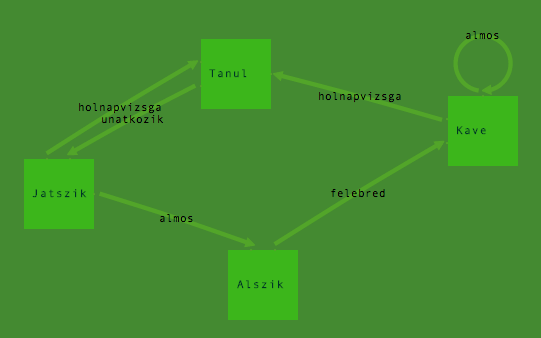
\includegraphics[width=100mm, keepaspectratio]{figures/tanulo.png}
\caption{A bemeneti diagram} 
\end{figure}


\begin{lstlisting}[caption=Az állapotgép kódgeneráló UnderscoreJS template-je]  

var sm = function() {

states = [

<% doc.entities.forEach(function(entity,i){
%>
  {"name": "<%= entity.title %>", 
   <%if(i==0){ %> "initial":true, <% }%>
  "events": {
    <% entity.connections_from.forEach(function(con){%>
        "<%=con.label%>":"<%=con.to%>",
    <%}) %>}
},<%
}) %>

]

 function StateMachine(states){
        this.states = states;
        this.indexes = {}; 
        for( var i = 0; i< this.states.length; i++){
            this.indexes[this.states[i].name] = i;
            if (this.states[i].initial){
                this.currentState = this.states[i];
            }
        }
        this.consumeEvent = function(e){
            if(this.currentState.events[e]){
                this.currentState = this.states[this.indexes[this.currentState.events[e]]] ;
                console.log(this.currentState.name);
            }
        }
        this.getStatus = function(){
            return this.currentState.name;
        }
    }
    return new StateMachine(states);
}

\clearpage

\end{lstlisting}



\begin{lstlisting}[caption=A generálás eredménye] 

var sm = function() {

states = [


  {"name": "Jatszik", 
    "initial":true, 
  "events": {"almos":"Alszik","holnapvizsga":"Tanul",}
},
  {"name": "Tanul", 
   
  "events": {"unatkozik":"Jatszik",}
},
  {"name": "Alszik", 
   
  "events": {"felebred":"Kave",}
},
  {"name": "Kave", 
   
  "events": {"holnapvizsga":"Tanul","almos":"Kave",}
},

]

 function StateMachine(states){
        this.states = states;
        this.indexes = {}; 
        for( var i = 0; i< this.states.length; i++){
            this.indexes[this.states[i].name] = i;
            if (this.states[i].initial){
                this.currentState = this.states[i];
            }
        }
        this.consumeEvent = function(e){
            if(this.currentState.events[e]){
                this.currentState = this.states[this.indexes[this.currentState.events[e]]] ;
                console.log(this.currentState.name);
            }
        }
        this.getStatus = function(){
            return this.currentState.name;
        }
    }
    return new StateMachine(states);
}

\end{lstlisting}


\label{page:last}
\end{document}
